%%%%%%%%%%%%%%%%%%%%%%%%%%%%%%%%%%%%%%%%%
% University/School Laboratory Report
% LaTeX Template
% Version 3.1 (25/3/14)
%
% This template has been downloaded from:
% http://www.LaTeXTemplates.com
%
% Original author:
% Linux and Unix Users Group at Virginia Tech Wiki 
% (https://vtluug.org/wiki/Example_LaTeX_chem_lab_report)
%
% License:
% CC BY-NC-SA 3.0 (http://creativecommons.org/licenses/by-nc-sa/3.0/)
%
%%%%%%%%%%%%%%%%%%%%%%%%%%%%%%%%%%%%%%%%%

%----------------------------------------------------------------------------------------
%	PACKAGES AND DOCUMENT CONFIGURATIONS
%----------------------------------------------------------------------------------------

\documentclass{ctexart}

\usepackage[version=3]{mhchem} % Package for chemical equation typesetting
\usepackage{siunitx} % Provides the \SI{}{} and \si{} command for typesetting SI units
\usepackage{graphicx} % Required for the inclusion of images
\usepackage{natbib} % Required to change bibliography style to APA
\usepackage{amsmath} % Required for some math elements 
%\usepackage{showframe} % for showing page frames


\setlength\parindent{0pt} % Removes all indentation from paragraphs

\renewcommand{\labelenumi}{\alph{enumi}.} % Make numbering in the enumerate environment by letter rather than number (e.g. section 6)

%\usepackage{times} % Uncomment to use the Times New Roman font

%==========pesusdo codes
\usepackage[linesnumbered,boxed]{algorithm2e}
%\renewcommand{\algorithmcfname}{算法}
\renewcommand{\repeat}{Repeat}

%==========citation===========
%\usepackage{cite}
\usepackage{url}


% ==========添加首行缩进,两个字符===========
\usepackage{indentfirst}
\setlength{\parindent}{2em}
% ==========强制图片位置===========
\usepackage{float}

% ==========特殊数学符号===========
\usepackage{mathtools}
\usepackage{dsfont}
\usepackage{amsfonts}
% ==========列表===========
\usepackage{enumerate}

%----------------------------------------------------------------------------------------
%	DOCUMENT INFORMATION
%----------------------------------------------------------------------------------------

\title{Naive Bayes} % Title

%\author{fengmi \textsc{Feng}} % Author name

\author{Mia Feng} % Author name

\date{\today} % Date for the report

\begin{document}

\maketitle % Insert the title, author and date

%\begin{center}
%\begin{tabular}{l r}
%Date Performed: & January 1, 2012 \\ % Date the experiment was performed
%Partners: & James Smith \\ % Partner names
%& Mary Smith \\
%Instructor: & Professor Smith % Instructor/supervisor
%\end{tabular}
%\end{center}

% If you wish to include an abstract, uncomment the lines below
% \begin{abstract}
% Abstract text
% \end{abstract}

%----------------------------------------------------------------------------------------
%	SECTION 1
%----------------------------------------------------------------------------------------

\section{概述}
Naive Bayes:监督学习,生成式模型。用于分类,朴素指的是各特征条件独立\cite{LiHang:Statistic}。用于垃圾邮件分类等。
%To determine the atomic weight of magnesium via its reaction with oxygen and to study the stoichiometry of the reaction (as defined in \ref{definitions}):

求解目标:分类,以后验概率最大时对应的类别作为预测分类结果。
\begin{equation}
y=\arg\max\limits_{c_k}P\big(Y=c_k\big)\prod\limits_{j=1}^{n}P\big(X_j=x_j|Y=c_k\big)
\end{equation}

求解思路:最大化后验概率,或者说省略分母不看后最大化似然,取后验概率最大或者似然值最大对应的类标作为预测类标。Concretely, 分别计算各类别出现概率$P\big(Y=c_k\big),k=1,2,\cdots,m$;分别计算各类别下对应特征出现的概率$P\big(X=x_j|Y=c_k\big),j=1,2,\cdots,n,k=1,2,\cdots,m$;按公式$\big(1\big)$预测类标。
求解方法:MAP或者最大化似然。


% If you have more than one objective, uncomment the below:
%\begin{description}
%\item[First Objective] \hfill \\
%Objective 1 text
%\item[Second Objective] \hfill \\
%Objective 2 text

\subsection{推导}
\label{derivations}
\begin{description}
\item[推导]
取$I$为示性函数。$a_l$表示$X$的第$l$个特征。样本有n个。类标m个,特征s个。
\begin{equation}
P\big(Y=c_k\big)=\frac{\sum\limits_{i=1}^{n}I\big(y_i=c_k\big)}{n},k=1,2,\cdots,m
\end{equation}

\begin{equation}
P\big(X_j=a_{jl}|Y=c_k\big)=\frac{\sum\limits_{i=1}^{n}I\big(x_i^j=a_{jl},y_i=c_k\big)}{\sum\limits_{i=1}^{n}I\big(y_i=c_k\big)}
\end{equation}
其中,$i=1,2,\cdots,n$,$l=1,2,\cdots,s$,$k=1,2,\cdots,m$
\end{description}

%----------------------------------------------------------------------------------------
%	SECTION 2
%----------------------------------------------------------------------------------------

\section{算法实现}
见CS229\cite{stanf:cs229}
%
\begin{enumerate}[1.]
\item 随机初始化cluster centroids $\mu_1,\mu_2,\cdots,\mu_k\in\mathbb{R}^n$
\item 迭代直至收敛\{

对于每一个样例$i$,计算类标
\begin{equation}
c^{\left(i\right)}\coloneqq \arg\min\limits_{j}\big\| x^{\left(i\right)}-\mu_{j}\big\|^2
\end{equation}
对于每一个类$j$,更新cluster centroids:
\begin{equation}
\mu_j \coloneqq \frac{\sum\limits_{i=1}^{m}\mathds{1}\left\{c^{\left(i\right)}=j\right\}x^{\left(i\right)}}{\sum\limits_{i=1}^{m}\mathds{1}\left\{c^{\left(i\right)}=j\right\}}
\end{equation}
\}
\end{enumerate}

%----------------------------------------------------------------------------------------
%	SECTION 3
%----------------------------------------------------------------------------------------
%
\section{Implementation}
聚类测试:数据在data.csv
\begin{figure}[H]
\begin{center}
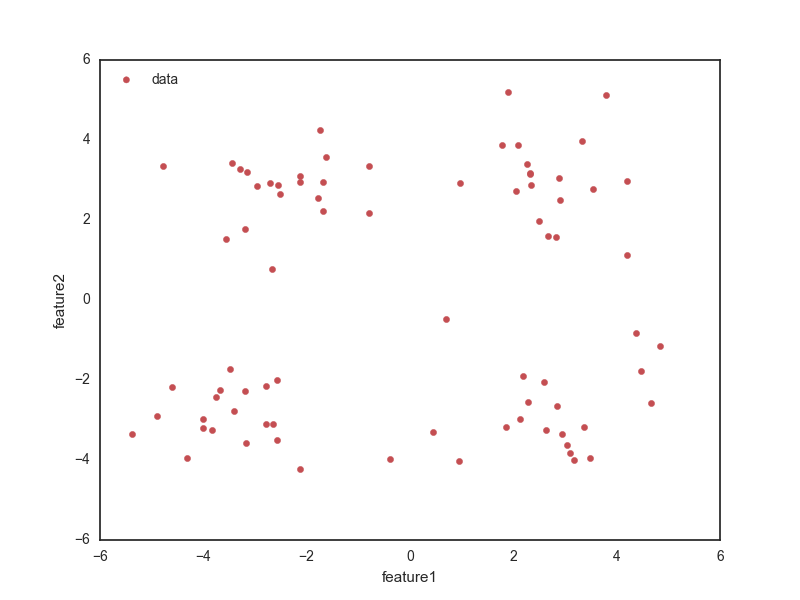
\includegraphics[width=0.8\textwidth]{fig/raw.png} % Include the image placeholder.png
\caption{训练数据}
\end{center}
\end{figure}

\begin{figure}[H]
\begin{center}
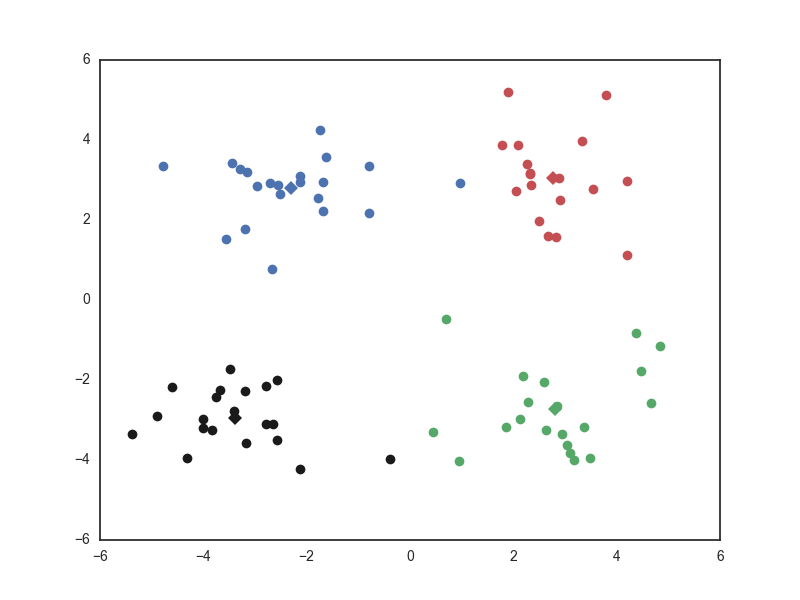
\includegraphics[width=0.8\textwidth]{fig/iter-01.png} % Include the image placeholder.png
\caption{kmeans运行结果,iter=1,$k$=4。菱形标记聚类中心,点标记数据}
\end{center}
\end{figure}


\begin{figure}[H]
\begin{center}
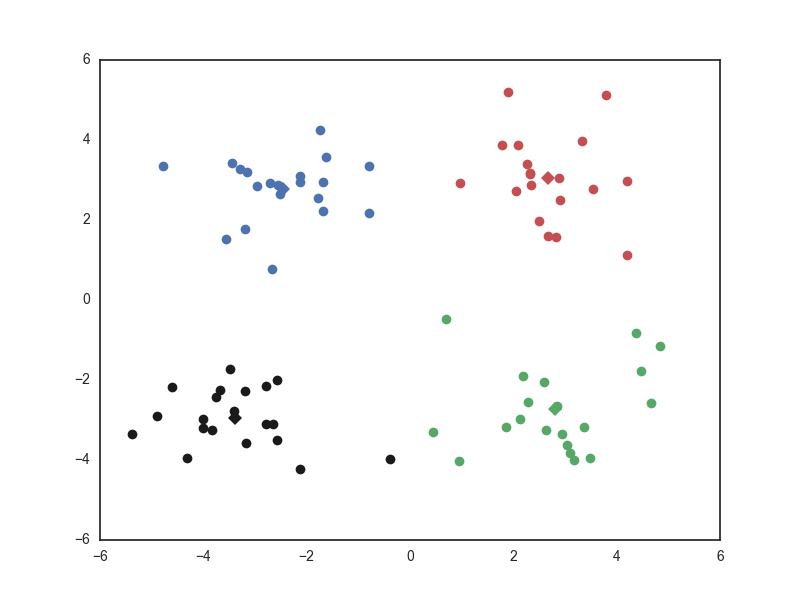
\includegraphics[width=0.8\textwidth]{fig/iter-02.png} % Include the image placeholder.png
\caption{kmeans运行结果,iter=2,$k$=4。菱形标记聚类中心,点标记数据}
\end{center}
\end{figure}


\begin{figure}[H]
\begin{center}
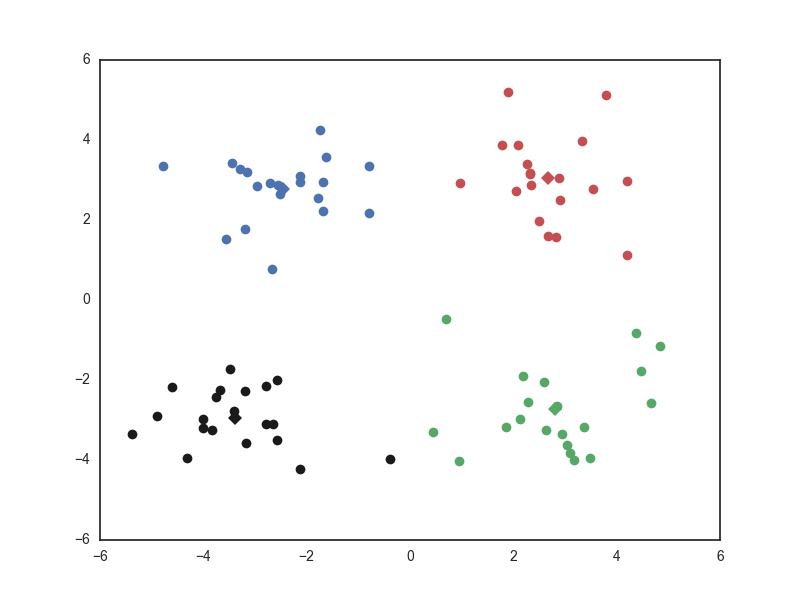
\includegraphics[width=0.8\textwidth]{fig/iter-03.png} % Include the image placeholder.png
\caption{kmeans运行结果,iter=3,$k$=4。菱形标记聚类中心,点标记数据}
\end{center}
\end{figure}

%%----------------------------------------------------------------------------------------
%%	SECTION 4
%%----------------------------------------------------------------------------------------
%
%\section{Results and Conclusions}
%
%The atomic weight of magnesium is concluded to be \SI{24}{\gram\per\mol}, as determined by the stoichiometry of its chemical combination with oxygen. This result is in agreement with the accepted value.
%
%\begin{figure}[h]
%\begin{center}
%\includegraphics[width=0.65\textwidth]{placeholder} % Include the image placeholder.png
%\caption{Partial Gradient of $L_\big(\theta \big)$}
%\end{center}
%\end{figure}
%
%%----------------------------------------------------------------------------------------
%%	SECTION 5
%%----------------------------------------------------------------------------------------
%
%\section{Discussion of Experimental Uncertainty}
%
%The accepted value (periodic table) is \SI{24.3}{\gram\per\mole} \cite{Smith:2012qr}. The percentage discrepancy between the accepted value and the result obtained here is 1.3\%. Because only a single measurement was made, it is not possible to calculate an estimated standard deviation.
%
%The most obvious source of experimental uncertainty is the limited precision of the balance. Other potential sources of experimental uncertainty are: the reaction might not be complete; if not enough time was allowed for total oxidation, less than complete oxidation of the magnesium might have, in part, reacted with nitrogen in the air (incorrect reaction); the magnesium oxide might have absorbed water from the air, and thus weigh ``too much." Because the result obtained is close to the accepted value it is possible that some of these experimental uncertainties have fortuitously cancelled one another.
%
%%----------------------------------------------------------------------------------------
%%	SECTION 6
%%----------------------------------------------------------------------------------------
%
%\section{Answers to Definitions}
%
%\begin{enumerate}
%\begin{item}
%The \emph{atomic weight of an element} is the relative weight of one of its atoms compared to C-12 with a weight of 12.0000000$\ldots$, hydrogen with a weight of 1.008, to oxygen with a weight of 16.00. Atomic weight is also the average weight of all the atoms of that element as they occur in nature.
%\end{item}
%\begin{item}
%The \emph{units of atomic weight} are two-fold, with an identical numerical value. They are g/mole of atoms (or just g/mol) or amu/atom.
%\end{item}
%\begin{item}
%\emph{Percentage discrepancy} between an accepted (literature) value and an experimental value is
%\begin{equation*}
%\frac{\mathrm{experimental\;result} - \mathrm{accepted\;result}}{\mathrm{accepted\;result}}
%\end{equation*}
%\end{item}
%\end{enumerate}

%----------------------------------------------------------------------------------------
%	BIBLIOGRAPHY
%----------------------------------------------------------------------------------------
%
% 注意一定要在文中引用才不会出错(至少引用一个)
\bibliographystyle{plain}
\bibliography{bib//nb}

%----------------------------------------------------------------------------------------


\end{document}